\documentclass[11pt]{article}

\usepackage{common}
\usepackage{subcaption}
\title{Practical 1: Predicting the Efficiency of Organic Photovoltaics\\Repository: https://github.com/tongbaojia/pubcs181}
\author{Baojia Tong, baojia.tong@cern.ch \\ Yuliya Dovzhenko, dovzhenko@g.harvard.edu \\ Alan Le Goallec, alanlegoallec@g.harvard.edu}
\begin{document}
\maketitle{}


\noindent For this first practical, we were asked to predict how suitable 800K different molecules would be
for use in solar panels. The relevant physical property of these molecules that we tried to predict
was the "gap" value, defined by the difference in energy between the highest and the lowest occupied molecular orbital.
To do this, we had access to a 100K samples training set. The features that we used were all computed from the 
string representation of the molecule, using a package called RDkit.
We will first present how we preprocessed the data, and we will then describe the different machine algorithms that we
used and the results we obtained.


\section{Technical Approach: Preprocessing}

  \subsection{Removing weakly correlated features}
    The samples that we were given contained 256 features precalculated using RDkit.
    The first step was to check how many of these features contain significant information, and to remove weakly correlated features.
    In theory, extra useless features should not prevent us from finding a good model, as they can easily
    be ignored if necessary (by setting their coefficient to 0 for a linear regression for example). However,
    they can slow down the tuning process of the model, and keep us from exploring some models or some non linear
    feature transformations within a reasonable time. \\
    To filter the features that we judged useless, we first looked at their correlation with the output that we were
    trying to predict (the gap values), and got rid of every feature that was not at least 10\% correlated.
    It appeared that the vast majority of the features were poorly correlated with our outcome of interest.
    We are well aware that in theory a feature could have an impressive predictive power while showing a 0\% correlation with
    the output (for example if the correlation is +1 on half of the samples, and -1 with the other half, which a decision tree could exploit
    if these two halves can be separated using the value of one of the predictors),
    but we find it unlikely here and we are willing to take the risk to loose some information.
    After this first preprocessing step, we were left with only 7 predictors.
    Note: to gain some time, we only used 20\% of the data to determine which features we should use.

  \subsection{Adding chemistry features with rdchem}
  The simplest, analytically-solvable analogy to our DFT problem is problem of calculating the energy spectrum of a Hydrogen atom in introductory quantum mechanics.  The difference between the $n$'th and $(n+1)$'th energy level is found to be
  
  \begin{equation}
  \Delta E_n \frac{Zk_e e^2}{2r_n},
  \end{equation} 
where $Z$ is the atomic number, and $r_n$ is the Bohr radius, which is a function of the energy level number and a few known quantities. Our case of a multi-atom molecule is more complicated because it involves electron-electron interactions (in chemistry, they are described as bonds). However, the atomic numbers of the constituent atoms will still be important. In rdkit.Chem, we have the following properties which together hint at this information: molecular weight, average molecular weight, number of heavy atoms and number of atoms). The size of the gap also depends on the chemical potential, which is roughly related to the  average number of electrons per atom. Therefore, we will be interested in properties that have to do with the number of electrons. We found the following usefull properties found in rdkit Descriptor package: number of heavy atoms, number of atoms, molecular weight, average molecular weight of heavy atoms, average molecular weight, number of valence electrons and number of radical electrons.

RMSE comparison with a benchmark: 
\begin{itemize}
\item{Without extra features: LR RMSE = 0.3047;  RF RMSE = 0.2874}
\item{With extra features:LR RMSE = 0.2252;  RF RMSE = 0.2273}
\end{itemize}

  \subsection{Adding non linear terms}
  
    To capture the potential interactions between the different predictors, we added the interaction terms (the products between the
    different predictors). We also computed the quadratic terms.
    This was only a realistic idea because of the previous filtering of the not so useful features.
    
    \subsection{Scaling}
    Not all the features have the same order of magnitude. Because it is not intuitive that the unit in which a feature is expressed
    should influence its ability to affect prediction, and because we want all the features to be equally able to affect the prediction,
    we normalized all our predictors. (Features with a large range affect some models more than features with smaller range. Decision trees
    are not affected, but linear regression is, for example.) \\
    We made sure to do that by only looking at the training set, and then applied the same transformations to the columns of the testing set.
    
    
\section{Technical Approach: Models}
    \subsection{Main model: Regularized Linear Regression}
    We chose to focus on Linear Regression, and regularized it in different ways. \\
    We first used LASSO as a penalty: LASSO adds a regulariation term in norm 1, which encourages a sparse model: the total sum of the
    coefficients tends to remain small, but it does not matter how this quantity is spread between the features.
    So if some features are correlated, one of them will tend to carry the weight of the others and see its coefficient increase, while the 
    other features see their coefficient set to zero. \\
    We then used RIDGE regression: this time the penalty term is in norm 2, so big coefficients are even more penalized: not only is the sum
    of the coefficient encouraged to remain small, but individual coefficient tend to do the same. So if several features are
    correlated, the model will tend to distribute the total amount of coefficient between the features. Therefore the resulting model is not
    as sparse as the one generated by LASSO regression. \\
    Finally we used an elastic net. An elastic net is basically the combination between a LASSO and a RIDGE regression, since an extra
    hyperparameter is introduced: if this parameter is 0, the elastic net is equivalent to a LASSO. If this parameter is 1, it is equivalent
    to a RIDGE. For every value in between 0 and 1, the model is trying a weighted compromise between LASSO and RIDGE regularization.
    So an elastic net basically introduces an extra hyperparameter to do model selection between LASSO, RIDGE, and their combinations.
    
    \subsection{Partial Least Squares}
Since we are dealing with a large sparse matrix (many zeros in the original features), we decided to explore dimension reduction. In particular, we focused on the Partial Least Squares (PLC) algorithm, which projects the data onto planes of greatest variance. These planes are referred to as principal components, and they represent the degree of variability that exists in the data. We have already seen in the Preprocessing section that not all features are equally important in predicting the data. It would be a logical step to look for combinations of features which together represent one meaningful aspect of the data. 

The results are plotted in figure \ref{fig:PCL}.  The three plots correspond to PLC results different sets of data: (a) original data, (b) original data with additional chemistry features, and (c) truncated data with chemistry features. For comparison, all three tests were performed on the same subsets of the data, with 40,000 molecules used for training and 8,000 molecules used for testing. 

All three plots show the RMSE converging toward a minimum value, however this does not happen at the same number of principal components. Furthermore, the value of the RMSE plateau is different in different cases. With only original data, the error is ~0.3, comparable with the LR benchmark. This indicates to us that the features in the data can be accureately represented by a little over 10 components, and still fully capture the linear aspects of the model. However, the fact that RMSE plateaus at 0.3 does not mean that we have found the optimal model. It merely indicates that there are non-linear features present in the data, which we cannot identify with a principal component analysis. 

The best result using PLC is achieved on the truncated data set with additional chemistry features in \ref{fig:PLC} (c), and the RMSE converges after ~30 components. This confirms to us that chemistry features do in fact provide new information not present in the original data. The new information could be independent from the original features, or it could contain non-linear functions of the original data. 

\begin{figure}[] 
\begin{subfigure}[t]{0.5\textwidth}
        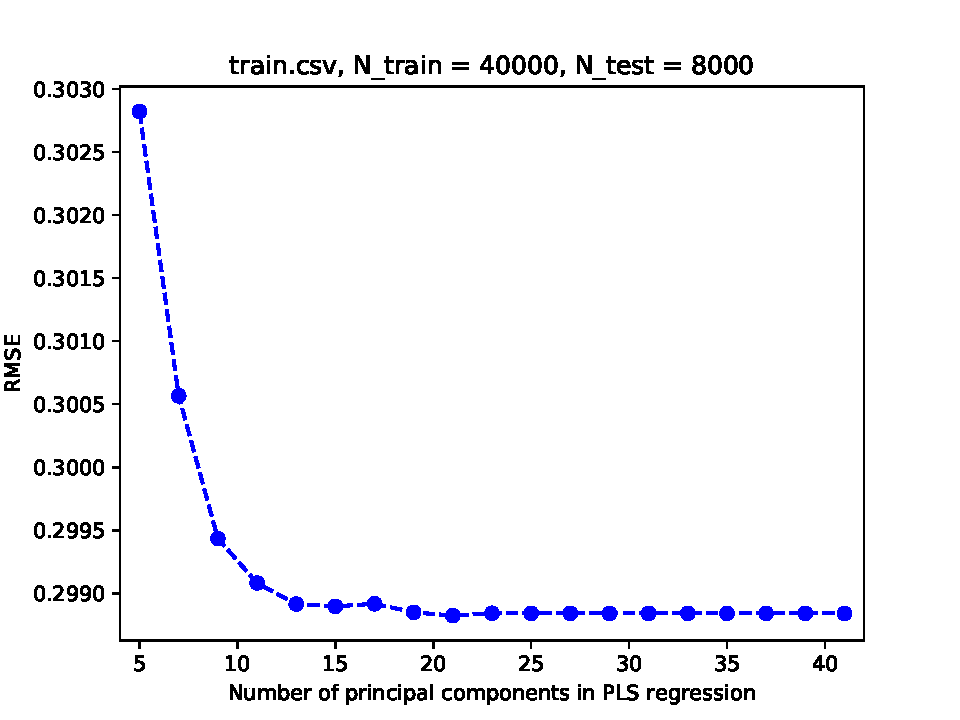
\includegraphics[width=\textwidth]{train_N_train_40000_N_test_8000.pdf}
    \end{subfigure}
    \begin{subfigure}[t]{0.5\textwidth}
        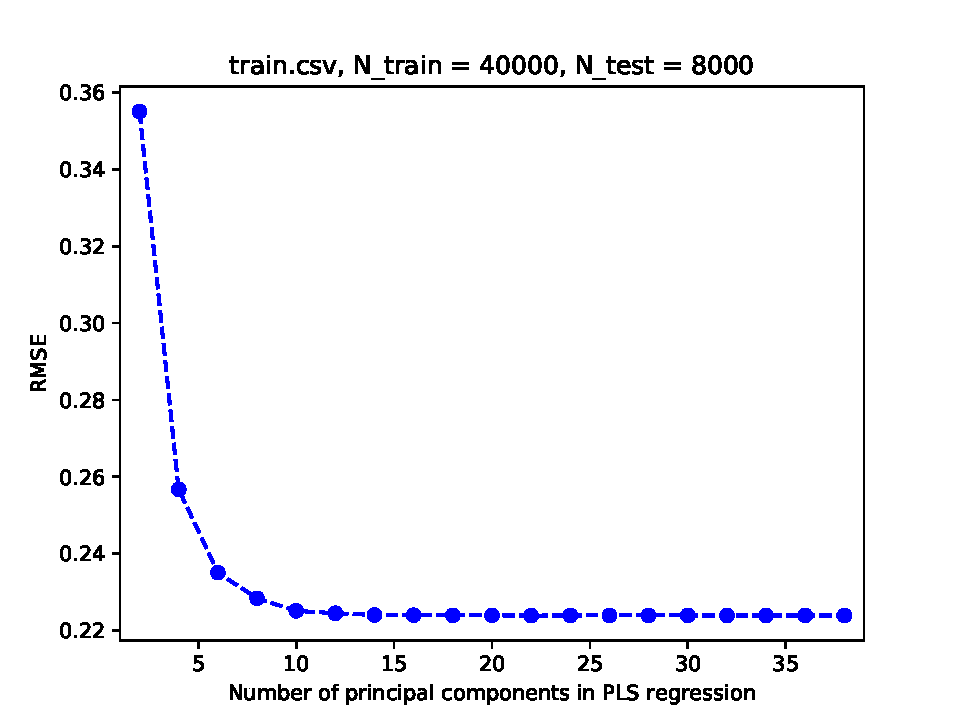
\includegraphics[width=\textwidth]{train_rdkit_N_train_40000_N_test_8000.pdf}
    \end{subfigure}
    \\
        \begin{subfigure}[t]{0.5\textwidth}
        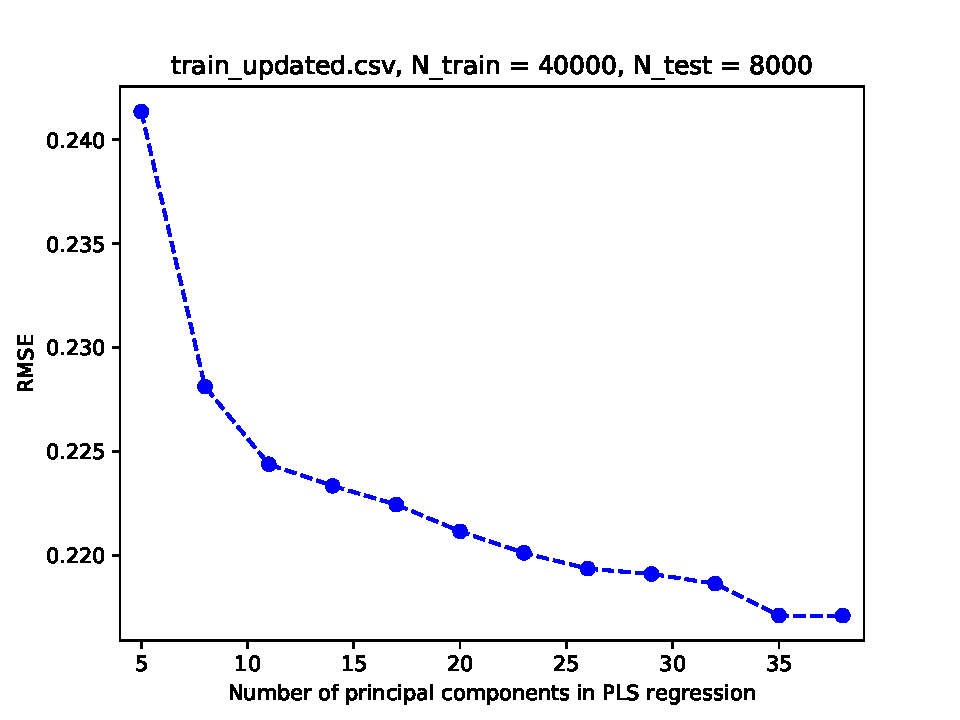
\includegraphics[width=\textwidth]{train_updated_N_train_40000_N_test_8000.pdf}
    \end{subfigure}
        \caption{(a) Results of PCL trained on the original data (no extra features). The RMSE is plotted as function of the number of principal components specified in the fitting. (b) Similar to (a), but but after adding rdkit features to the original data. (c) Similar to (a), but using the truncated dataset with chemistry features. }
            \label{fig:PCL}
\end{figure}

\section{Technical Approach: Validation}
    \subsection{Split}
    To develop and validate our models quickly without having to submit them on kaggle, we split our training data in two sets, that
    we used as training and testing sets. (which \% did we use? 50/50 split?)
    Note: In order to accelerate the troubleshooting process, we first ran models on a small subset of our data (training and testing sets
    of 10k samples, and then tuned them and evaluated using all the data we had.
    
    \subsection{Cross Validation}


\section{Results}


\section{Discussion}

+ Future directions
add other features
CV? 

\end{document}

